\section{Regresión lineal simple y múltiple}
\begin{itemize}[label=\color{red}\textbullet, leftmargin=*]
	\item \color{lightblue}Introducción
\end{itemize}
\lb{Objetivo:} predecir una variable numérica a partir de $k$ variables numéricas (variables predictoras) minimizando el error en la predicción.

Para ello necesitamos disponer de una muestra en la que se conozcan dichas variables (aprendizaje supervisado), esta muestra se usará para elegir el mejor modelo y para validar su fiabilidad.
\begin{itemize}[label=\color{red}\textbullet, leftmargin=*]
	\item \color{lightblue}Planteamiento
\end{itemize}
Se trata de predecir el valor (numérico) de una \va (v.a.) $Y$ a partir de unas variables predictoras $X_1,\dots,X_k$.

Para ello usaremos una función predictora lineal \[ h_\theta(x_1,\dots,x_k)\coloneq\theta_0+\theta_1x_1+\cdots+\theta_kx_k, \] donde $\theta=(\theta_0,\dots,\theta_k)'\in\R^{k+1}$ serán los parámetros del modelo que se deben elegir de forma que la estimación de $Y$ sea óptima (el error sea mínimo).
\begin{itemize}[label=\color{lightblue}$\to$]
\item Una sola variable predictora $\longrightarrow$ \lb{Regresión lineal simple}.
\item Más de una variable predictora $\longrightarrow$ \lb{Regresión lineal múltiple}.
\end{itemize}

\subsection{Estimación de los parámetros}
\subsubsection{Muestra}
Para ello necesitamos disponer de una muestra (\lb{training sample}) de esas $k+1$ variables sobre $n$ individuos.

Una realización de la muestra se denotará como \[ \left(x_1^{(i)},\dots,x_k^{(i)},y^{(i)}\right),\quad i=1,\dots,n, \] que equivale a la notación introducida en el tema anterior \[ (x_{i,1},\dots,x_{i,k},y_i),\quad i=1,\dots,n. \]
Los datos se representan en forma de tabla:
\[ \begin{array}{cccccc}
i & x_1 & x_2 & \cdots & x_k & y \\ \hline
\mathbf{o}_1 & x_1^{(1)} & x_2^{(1)} & \cdots & x_k^{(1)} & y_1 \\
\cdots & \cdots & \cdots & \cdots & \cdots & \cdots \\
\mathbf{o}_i & x_1^{(i)} & x_2^{(i)} & \cdots & x_k^{(i)} & y_i \\
\cdots & \cdots & \cdots & \cdots & \cdots & \cdots \\
\mathbf{o}_n & x_1^{(n)} & x_2^{(n)} & \cdots & x_k^{(n)} & y_n \\ \hline
\end{array}\qquad\begin{array}{cccccc}
i & x_1 & x_2 & \cdots & x_k & y \\ \hline
\mathbf{o}_1 & x_{1,1} & x_{1,2} & \cdots & x_{1,k} & y_1 \\
\cdots & \cdots & \cdots & \cdots & \cdots & \cdots \\
\mathbf{o}_i & x_{i,1} & x_{i,2} & \cdots & x_{i,k} & y_i \\
\cdots & \cdots & \cdots & \cdots & \cdots & \cdots \\
\mathbf{o}_n & x_{n,1} & x_{n,2} & \cdots & x_{n,k} & y_n \\ \hline
\end{array} \]

\subsection{Conjunto de datos \textbf{\texttt{USArrests}}}

\subsubsection*{Cargamos los datos}
Podemos visualizar los datos con \code{view(d)} y las primeras filas con \code{head(d)}.

\begin{lstlisting}
d <- USArrests
head(d, n = 6)
\end{lstlisting}

\begin{verbatim}
##            Murder Assault UrbanPop Rape
## Alabama      13.2     236       58 21.2
## Alaska       10.0     263       48 44.5
## Arizona       8.1     294       80 31.0
## Arkansas      8.8     190       50 19.5
## California    9.0     276       91 40.6
## Colorado      7.9     204       78 38.7
\end{verbatim}
\subsubsection*{¿Qué información está recogida en el conjunto de datos?}
Con la instrucción \code{help(USArrests)} conocemos qué información está contenida en el conjunto:
\begin{itemize}
\item \code{Murder:} Ratios de arrestos por asesinatos por cada $100\,000$ residentes en cada uno de los 50 estados de la unión.
\item \code{Assault:} Ratios de arrestos por agresión por cada $100\,000$ residentes en cada uno de los 50 estados de la unión.
\item \code{UrbanPop:} Porcentaje de población que vive en áreas urbanas.
\item \code{Rape:} Ratios de arrestos por violación por cada $100\,000$ residentes en cada uno de los 50 estados de la unión.
\end{itemize}
\subsubsection{Objetivo}

Predecir el ratio de arrestos por asesinatos ($Y=$\code{Murder}) en función de la variable $X=$\code{UrbanPop}.

\begin{wrapfigure}[3]{r}{0.4\textwidth}

\begin{tikzpicture}
	\node[red, draw=red, fill=red!10, line width=1.5, text width=\linewidth] {Podemos observar que no parece existir ninguna relación entre las variables \texttt{Murder} y \texttt{UrbanPop} por lo que la predicción no será muy buena.};
\end{tikzpicture}
\end{wrapfigure}

Para visualizar la relación entre estas variables podemos representarlas situando $X$ en el eje horizontal e $Y$ en el vertical.

\begin{lstlisting}
x <- d$UrbanPop #Elegimos x
y <- d$Murder #Elegimos y
plot(x, y, xlab = 'UrbanPop', ylab = 'Murder')
\end{lstlisting}

\begin{center}
\includegraphics[scale=0.7]{"Temas/Imágenes/Tema 2/000005"}
\end{center}

\newpage

\begin{wrapfigure}[4]{r}{0.4\textwidth}

\begin{tikzpicture}
	\node[red, draw=red, fill=red!10, line width=1.5, text width=\linewidth] {Ahora sí se aprecia una relación lineal (creciente entre ambas variables.)};
\end{tikzpicture}
\end{wrapfigure}

Si usamos como predictor la variable \code{Assault} y representamos gráficamente:

\begin{lstlisting}
x <- d$Assault #Elegimos x
y <- d$Murder #Elegimos y
plot(x, y, xlab = 'Assault', ylab = 'Murder')
\end{lstlisting}

\begin{center}
\includegraphics[scale=0.7]{"Temas/Imágenes/Tema 2/000010"}
\end{center}

\subsubsection{Matriz de gráficos}
Podemos representar conjuntamente todas las variables con gráficos bidimensionales para cada pareja de variables.

\begin{lstlisting}
plot(d)
\end{lstlisting}

\begin{center}
\includegraphics[scale=0.7]{"Temas/Imágenes/Tema 2/000002"}
\end{center}
\subsubsection{Resumen numérico de las variables}
Podemos obtener los estadísticos descriptivos de estas variables con \code{summary(d)} que incluyen los extremos (mínimo y máximo), los cuartiles, la mediana y la media.
\begin{lstlisting}
summary(d)
\end{lstlisting}
\begin{verbatim}
##      Murder          Assault         UrbanPop          Rape
##  Min.   : 0.800   Min.   : 45.0   Min.   :32.00   Min.   : 7.30
##  1st Qu.: 4.075   1st Qu.:109.0   1st Qu.:54.50   1st Qu.:15.07
##  Median : 7.250   Median :159.0   Median :66.00   Median :20.10
##  Mean   : 7.788   Mean   :170.8   Mean   :65.54   Mean   :21.23
##  3rd Qu.:11.250   3rd Qu.:249.0   3rd Qu.:77.75   3rd Qu.:26.18
##  Max.   :17.400   Max.   :337.0   Max.   :91.00   Max.   :46.00
\end{verbatim}
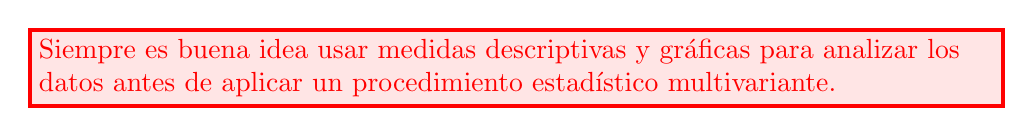
\begin{tikzpicture}
	\node[red, draw=red, fill=red!10, line width=1.5, text width=\linewidth] {Siempre es buena idea usar medidas descriptivas y gráficas para analizar los datos antes de aplicar un procedimiento estadístico multivariante.};
\end{tikzpicture}
\subsubsection{Estimación de las varianzas y covarianzas}
Para calcular una estimación de las varianzas y covarianzas utilizaremos la función \code{var} (\code{R} obtiene las cuasivarianzas).

\begin{lstlisting}
#calculo directo de la varianza y cuasivarianza para Murder
mu <- mean(d$Murder)
n <- length(d)
hat_sigma = sum((d$Murder-mu)^ 2)/n #varianza muestral
S = sum((d$Murder-mu)^ 2)/(n-1) #cuasivarianza muestral
#calculo de la matriz de covarianzas
var(d)
\end{lstlisting}

\begin{verbatim}
##              Murder   Assault   UrbanPop      Rape
## Murder    18.970465  291.0624   4.386204  22.99141
## Assault  291.062367 6945.1657 312.275102 519.26906
## UrbanPop   4.386204  312.2751 209.518776  55.76808
## Rape      22.991412  519.2691  55.768082  87.72916
\end{verbatim}

\subsubsection{Modelo completo}

Podemos incluir todas las variables en el modelo considerado \[ h_\theta=\theta_0+\theta_1\text{Assault}+\theta_2\text{UrbanPop}+\theta_3\text{Rape} \]donde $\theta=(\theta_0,\theta_1,\theta_2,\theta_3)'\in\R^4$ son los parámetros del modelo que debemos ajustar para obtener las mejores aproximaciones posibles.

Los casos en los que solo usamos una variable están incluidos en este modelo haciendo que los parámetros de las otras variables sean cero.

También podemos intentar mejorar estas aproximaciones considerando otras funciones $h$ (no lineales).

\subsection{Regresión lineal simple}
\subsubsection{Modelo teórico}
Partiremos de un \vea $(X,Y)$.

\lb{Objetivo:} Construir una nueva variable $h(X)$ que se \lb{parezca} (aproxime) a $Y$.

Los errores (residuos) serán otra variable aleatoria \[ R=Y-h(X) \](notemos que pueden ser positivos o negativos).

Existen diversas reglas para determinar una función objetivo que mida cómo son esos errores y trate de minimizarlos.

La más usada es el denominado \lb{error cuadrático medio} (EMC) definido como: \[ EMC=E\left[(h(X)-Y)^2\right] \] (MSE, \lb{Mean Square Error})

\subsubsection{Función óptima}

Supongamos que $(X,Y)$ tiene una distribución absolutamente continua con función de densidad conjunta $f$ y marginales $f_X$ y $f_Y$.

Entonces se puede demostrar que la función $h$ que \lb{minimiza} el $EMC$ es \[ h_{\mathrm{opt}}(x)=E(Y|X=x)=\infi yf_{Y|X}(y|x)\dy, \]donde\[ f_{Y|X}(y|x)=f(x,y)|f_X(x), \] para tales $f_X(x)>0$, es la \lb{función de densidad condicionada} de $(Y|X=x)$.

Esta función se denomina \lb{curva de regresión} y es el mejor predictor de $Y$ dado $X$ según el $ECM$.
\subsection{Caso de normalidad}
El vector $(X,Y)$ tiene una distribución normal $\mathcal{N}_2(\mu,V)$:

$\mu=(\mu_1,\mu_2)'$ es el vector de medias ($A'$ representa la traspuesta de la matriz $A$), donde \[ \begin{array}{l}
\mu_1=\mu_X=E[X]\\
\mu_2=\mu_Y=[Y]
\end{array} \]
$V=\begin{pmatrix}
\sigma_{1,1} & \sigma_{1,2}\\
\sigma_{2,1} & \sigma_{2,2}\\
\end{pmatrix}$ es la matriz de varianzas-covarianzas, donde \[ \begin{array}{l}
\sigma_{1,1}=\sigma_X^2=\var(X)=E[(X-\mu_X)^2],\\
\sigma_{2,2}=\sigma_Y^2=\var(Y)=E[(Y-\mu_Y)^2],\\
\sigma_{1,2}=\sigma_{2,1}=\sigma_{X,Y}=\cov(X,Y)=E[(X-\mu_X)(Y-\mu_Y)].
\end{array} \]

Entonces la \lb{distribución condicionada} $(Y|X=x)$ se comporta también como una \lb{distribución normal}, \[ (Y|X=x)\longrightarrow \mathcal{N}_1(\overline{\mu},\overline{\sigma}^2), \] con \[ \begin{array}{c}
\begin{aligned}
h_{\mathrm{opt}}(x)=\overline{\mu}&=E(Y|X=x)=\mu_2+\dfrac{\sigma_{1,2}}{\sigma_{1,1}}(x-\mu_1)\\
&=\mu_Y+\dfrac{\cov(X,Y)}{\sigma_X^2}(x-\mu_X)
\end{aligned}\\
\overline{\sigma}^2=\var(Y|X=x)=\sigma_{2,2}-\dfrac{\sigma_{1,2}^2}{\sigma_{1,1}}=\sigma_Y^2-\dfrac{\cov(X,Y)^2}{\sigma_X^2}.
\end{array} \]

\begin{itemize}[label=\color{red}\textbullet, leftmargin=*]
	\item \color{lightblue}Observaciones
\end{itemize}
Bajo la hipótesis de normalidad, la \lb{curva de regresión} $h_{\mathrm{opt}}$ es siempre una \lb{recta} y la varianza $\overline{\sigma}^2$ no depende de $x$.

Los residuos condicionados $R_x=R|X=x$ también serán normales $R_x\longrightarrow \mathcal{N}(0,\overline{\sigma}^2)$ e idénticamente distribuidos.

La \lb{curva (recta) de regresión} para predecir $Y$ en función de $X$ se puede escribir como \[ \dfrac{y-\mu_Y}{\sigma_Y}=\rho_{X,Y}\dfrac{x-\mu_X}{\sigma_X}, \]donde $\rho_{X,Y}=\dfrac{\cov(X,Y)}{\sigma_X\sigma_Y}$ es el \lb{coeficiente de correlación lineal de Pearson}.

La recta siempre pasa por el punto $(\mu_X,\mu_Y)$.
\subsubsection{Coeficiente de correlación de Pearson}
\begin{itemize}[label=\color{red}\textbullet, leftmargin=*]
	\item \color{lightblue}Propiedades
\end{itemize}
El \lb{signo de la pendiente de la recta} de regresión siempre coincide con el signo de $\rho_{X,Y}$.

Se verifica que: \[ \overline{\sigma}^2=\sigma_Y^2-\dfrac{\cov(X,Y)^2}{\sigma_X^2\sigma_Y^2}\sigma_Y^2=(1-\rho_{X,Y}^2)\sigma_Y^2\ge0, \]por lo que $-1\le\rho_{X,Y}\le1$.

Cuando $\rho_{X,Y}=\pm1$ tendremos ajustes perfectos con residuos nulos.

La recta (curva) para predecir $X$ a partir de $Y$ se calcula de forma similar y no coincide con la curva para predecir $Y$ a partir de $X$ que acabamos de calcular salvo cuando $\rho_{X,Y}=\pm1$.
\subsection{Caso de no normalidad}
\begin{itemize}[label=\color{red}\textbullet, leftmargin=*]
	\item \color{lightblue}Observaciones
\end{itemize}
Para otras distribuciones bivariantes la curva de regresión no tiene por qué ser una recta.\\
Cuando $X$ e $Y$ sean independientes, $Y$ e $(Y|X=x)$ tienen la misma distribución y la curva óptima \[ h_{\mathrm{opt}}(x)=E(Y|X=x)=E(Y) \] es constante (por lo que también es una recta).
\begin{itemize}[label=\color{lightblue}$\to$]
\item En este caso el valor de $X$ no influye en la predicción sobre $Y$.
\item $\rho_{X,Y}=0$ (recta horizontal).
\end{itemize}
\subsection{Restricción sobre la función $h$}
En \textbf{Regresión Lineal Simple} supondremos que la función $h$ es una recta
\begin{itemize}
\item Limitamos nuestra función $h$ a una recta, es decir, \[ h_\theta(x)\coloneq\theta_0+\theta_1x \]
\item Usamos como criterio minimizar el ECM.
\item El objetivo será \[ \min_{\theta_0,\theta_1}J(\theta_0,\theta_1), \] donde \[ J(\theta_0,\theta_1)\coloneq E[(h_\theta(X)-Y)^2]=E[(\theta_0+\theta_1X+Y)^2] \]se conoce como \lb{función costo} y $J(\theta_0,\theta_1)\ge0$.
\begin{itemize}[label=\color{lightblue}$\to$]
\item Por lo tanto, se trata de minimizar una función costo
\end{itemize}
\end{itemize}
\subsection{Minimizar la función costo}
\subsubsection{Ecuaciones normales de la recta}
La función $J(\theta)$ es convexa por lo que tendrá un único mínimo que se puede obtener resolviendo el sistema \[ \begin{array}{l}
\dfrac{\partial J(\theta_0,\theta_1)}{\partial\theta_0}=2E[\theta_0+\theta_1X-Y]=0\\
\dfrac{\partial J(\theta_0,\theta_1)}{\partial\theta_1}=2E[(\theta_0+\theta_1X-Y)X]=0\\
\end{array} \]
Estas ecuaciones se conocen como \lb{ecuaciones normales}.

De la primera ecuación obtenemos \[ \theta_0=E(Y)-\theta_1E(X) \](con lo que la recta pasará por el punto formado con las medias).

De la segunda \[ \theta_0E(X)+\theta_1E(X^2)=E(XY) \]
Y sustituyendo la primera en la segunda, se obtiene \[ E(X)E(Y)-\theta_1E^2(X)+\theta_1E(X^2)=E(XY), \]es decir, \[ \theta_1\var(X)=\cov(X,Y), \]puesto que $\var(X)=E(X^2)-E^2(X)$ y $\cov(X,Y)=E(XY)-E(X)E(Y)$.

Con lo cual,
\begin{itemize}[label=\color{lightblue}$\to$]
\item $\hat{\theta}_1=\dfrac{\cov(X,Y)}{\var(X)}=\dfrac{\sigma_{X,Y}}{\sigma_X^2}$
\item $\hat{\theta}_0=E(Y)-\hat{\theta}_1E(X)=E(Y)-E(X)\dfrac{\cov(X,Y)}{\var(X)}=\mu_Y-\mu_X\dfrac{\sigma_{X,Y}}{\sigma_X^2}$
\end{itemize}
\subsection{Expresión de la recta}
\subsubsection{Recta de regresión para predecir $Y$ en función de $X$}
En el punto $(\hat{\theta}_0,\hat{\theta}_1)$ se alcanza el mínimo de la función $J$, \[ \min_{\theta_0,\theta_1}J(\theta_0,\theta_1)=J(\hat{\theta}_0,\hat{\theta}_1) \]
Expresión de la recta: \[ h_{\hat{\theta}}(x)=\mu_Y-\mu_X\dfrac{\sigma_{X,Y}}{\sigma_X^2}+\dfrac{\sigma_{X,Y}}{\sigma_X^2}x=\mu_Y+\dfrac{\sigma_{X,Y}}{\sigma_X^2}(x-\mu_X). \] (Note que la fórmula es la misma que la de la curva de regresión de la normal).

Otra expresión: \[ \dfrac{y-\mu_Y}{\sigma_Y}=\rho_{X,Y}\dfrac{x-\mu_X}{\sigma_X} \]donde $\rho_{X,Y}=\dfrac{\sigma_{X,Y}}{\sigma_X\sigma_Y}$ es el \lb{coeficiente de correlación lineal de Pearson}.

La \va \[ \hat{Y}=h_{\hat{\theta}}(X)=\hat{\theta}_0+\hat{\theta}_1X \]se usará para estimar $Y$.

Los residuos se definen como $R=Y-\hat{Y}$.

Se verifica:
\begin{itemize}[label=\color{lightblue}$\to$]
\item $E(\hat{Y})=E(Y)$
\item $E(R)=0$
\end{itemize}
\subsection{Descomposición de la varianza}
\subsubsection{Relaciones entre las varianzas}
Expresando $Y=\hat{Y}+R$, se tiene que: \[ \sigma_y=\var(Y)=\var(\hat{Y})+\var(R) \]
Puesto que \[ \begin{array}{c}
\var(\hat{Y})=\hat{\theta}_1^2\sigma_X^2=\dfrac{\sigma_{X,Y}P2}{\sigma_X^2}=\rho_{X,Y}^2\sigma_Y^2\\
\var(R)=\var(Y-\hat{\theta}_1X)=(1-\rho_{X,Y}^2)\sigma_Y^2.
\end{array} \]
Es decir, la información (varianza) contenida en $Y$ se descompone como \[ \sigma_Y^2=\rho_{X,Y}^2\sigma_Y^2+(1-\rho_{X,Y}^2)\sigma_Y^2. \]
\subsection{Coeficiente de determinación}
\begin{itemize}[label=\color{red}\textbullet, leftmargin=*]
	\item \color{lightblue}Definición
\end{itemize}
El \lb{coeficiente de determinación} $d_{X,Y}=\rho_{X,Y}^2$ es el porcentaje (en tanto por 1) de la información de $Y$ explicada por la recta de regresión (por relaciones lineales de $X$). Denotado habitualmente en los paquetes estadísticos por $R^2$.

Análogamente, $1-d_{X,Y}=1-\rho_{X,Y}^2$ indicaría la parte de $Y$ no explicada por esa recta y que se queda en el residuo.

Además, se tiene que \[ E(\hat{Y}R)=0, \] es decir, la variable que se obtiene con la recta de regresión y los residuos son incorrelados.

Bajo normalidad, ambas variables serán normales (por ser combinaciones lineales de $X$ e $Y$) y, por lo tanto, serán independientes.
\subsection{Inferencia y predicción}
\begin{itemize}[label=\color{red}\textbullet, leftmargin=*]
	\item \color{lightblue}Una muestra
\end{itemize}
En la práctica tanto la distribución conjunta (densidad) de $(X,Y)$ como todas esas medidas serán desconocidas por lo que tendrán que ser estimadas a partir de una muestra de esas variables (\lb{training sample}).

Si la muestra es grande, podemos extraer algunos datos (no usados en el cálculo de la recta) para comprobar cómo de fiables serán nuestras estimaciones.

La muestra se denotará como \[ \left(x^{(i)},y^{(i)}\right),\quad i=1,\dots,n, \]donde $n$ será el tamaño muestral.

Los datos de cada variable se representarán como columnas y todos lo datos como una matriz $D$.
\subsection{Función costo empírica}
\subsubsection{Objetivo}
Queremos aproximar los valores de $Y$ mediante una recta (función lineal) de $X$, es decir, \[ h_\theta\coloneq\theta_0+\theta_1x, \]donde $\mathbf{\theta}=(\theta_0,\theta_1)$ son parámetros desconocidos.

Para calcular estos parámetros minimizaremos una función coste empírica $J$ que nos mida el error cometido.

La más utilizada es el \lb{error cuadrático medio} (o una función proporcional a él), por ejemplo podemos considerar \[ J(\theta_0,\theta_1)\coloneq\dfrac{1}{2n}\sum_{i=1}^{n}\left(h_\theta\left(x^{(i)} \right) - y^{(i)}\right)^2=\dfrac{1}{2n}\sum_{i=1}^{n}\left(\theta_0+\theta_1x^{(i)}-y^{(i)}\right)^2 \]
El objetivo es minimizar esta función en $\R^2$.
\subsubsection{Diferenciar $J$}

Para obtener la solución exacta debemos diferencias $J$ con respecto a los parámetros obteniendo \[ \begin{array}{l}
	\dfrac{\partial}{\partial \theta_0}J(\theta_0,\theta_1)=\dfrac{1}{n}\sum_{i=1}^{n}\left(h\theta\left(x^{(i)}\right)-y^{(i)}\right)\\
	\dfrac{\partial}{\partial\theta_1}J(\theta_0,\theta_1)=\dfrac{1}{n}\sum_{i=1}^{n}\left(h_\theta\left(x^{(i)}\right)-y^{(i)}\right)x^{(i)}
\end{array} \]
Igualando a cero obtenemos las \lb{ecuaciones normales empíricas}:

$\begin{array}{l}
	\dfrac{\partial}{\partial \theta_0}J(\theta_0,\theta_1)=\dfrac{1}{n}\sum_{i=1}^{n}\left(h\theta\left(x^{(i)}\right)-y^{(i)}\right)=\dfrac{1}{n}\sum_{i=1}^{n}\left(\theta_0+\theta x^{(i)}-y^{(i)}\right)=0\\
	\dfrac{\partial}{\partial\theta_1}J(\theta_0,\theta_1)=\dfrac{1}{n}\sum_{i=1}^{n}\left(h_\theta\left(x^{(i)}\right)-y^{(i)}\right)x^{(i)}=\dfrac{1}{n}\sum_{i=1}^{n}\left(\theta_0+\theta_1x^{(i)}-y^{(i)}\right)x^{(i)}=0
\end{array}$
\subsubsection{Solución exacta}
De la primera ecuación, \[ \theta_0+\theta_1\overline{x}-\overline{y}=0 \]donde $\overline{x}=\dfrac{1}{n}\sum_{i=1}^{n}x^{(i)}$ e $\overline{y}=\dfrac{1}{n}\sum_{i=1}^{n}y^{(i)}$ son las medias muestrales de $x$ e $y$, respectivamente.

La solución óptima pasa por el punto medio $(\overline{x},\overline{y})$ (individuo promedio).

De la segunda, \[ \theta_0\overline{x}+\theta_1a(x,x)-a(x,y)=0,\] donde $a(x,x)=\dfrac{1}{n}\sum_{i=1}^{n}\left(x^{(i)}\right)^2$ y $a(x,y)=\dfrac{1}{n}\sum_{i=1}^{n}x^{(i)}y^{(i)}$.

Resolviendo este sistema de ecuaciones obtenemos \[ \theta_1\left(a(x,x)-(\overline{x})^2\right)=a(x,y)-\overline{xy} \]
Obtenemos: \[ \hat{\theta}_1=\dfrac{s_{x,y}}{s_x^2},\quad \hat{\theta}_0=\overline{y}-\hat{\theta}_1\overline{x}, \] donde $s_{x,y}=a(x,y)-\overline{xy}=\dfrac{1}{n}\sum_{i=1}^{n}x^{(i)}y^{(i)}-\overline{xy}=\dfrac{1}{n}\sum_{i=1}^{n}\left(x^{(i)}-\overline{x}\right)\left(y^{(i)}.\overline{y}\right)$ es la covarianza muestral y $s_x^2=a(x,x)-(\overline{x})^2=\dfrac{1}{n}\sum_{i=1}^{n}\left(x^{(i)}\right)^2-(\overline{x})^2=\dfrac{1}{n}\sum_{i=1}^{n}\left(x^{(i)}-\overline{x}\right)^2$ es la varianza muestral de $x$.

Supondremos que $s_x^2$ no es cero, es decir, que $x$ presenta más de un valor. Si no, el sistema tendría infinitas soluciones.

Puede comprobarse que $J$ es convexa y por lo tanto la solución que hemos obtenido de las ecuaciones normales empíricas es un mínimo local.
\begin{itemize}[label=\color{lightblue}$\to$]
	\item Además, como es único y $J$ es continua, se trata del único mínimo global.
\end{itemize}

\subsubsection*{¿Es un mínimo local?}
Las segundas derivadas parciales son \[ \begin{array}{l}
	D_{1,1}=\dfrac{\partial^2}{\partial\theta_0^2}J(\theta_0,\theta_1)=\dfrac{1}{n}\sum_{i=1}^{n}1=1\\
	D_{1,2}=\dfrac{\partial^2}{\partial\theta_0\theta_1}J(\theta_0,\theta_1)=\dfrac{1}{n}\sum_{i=1}^{n}x^{(i)}=\overline{x}\\
	D_{2,2}=\dfrac{\partial}{\partial\theta_1^2}J(\theta_0,\theta_1)=\dfrac{1}{n}\sum_{i=1}^{n}\left(x^{(i)}\right)^2=a(x,x)
\end{array} \]
Se verifica que $D_{1,1}=1>0$ y si $D=(D_{i,j})$ es la matriz con esas derivadas, tenemos \[ |D|=\begin{vmatrix}
	1 & \overline{x}\\
	\overline{x} & a(x,x)
\end{vmatrix}=a(x,x)-(\overline{x})^2=s_x^2>0 \]por lo que el punto sería un mínimo local de $J$.


\begin{tikzpicture}
	\node[red, draw=red, fill=red!10, line width=1.5, text width=\linewidth] {
	Como es el único mínimo local en $\R$ y $J$ es continua, será el único mínimo global.

	La solución óptima empírica coincide con la que obtendríamos sustituyendo en la solución teórica las medias, varianzas y covarianzas por sus estimaciones.
	};
\end{tikzpicture}
\subsection{Regresión lineal múltiple}
\subsubsection{Modelo teórico}
En el caso general queremos \lb{predecir} $Y$ (o $X_{k+1}$) a partir de $k$ variables $X_1,\dots,X_k$ (sobre el mismo espacio de probabilidad).

En el modelo lineal queremos construir una función \[ h_\theta(x_1,\dots,x_k)\coloneq\theta_0+\theta_1x_1+\cdots+\theta_kx_K, \]de forma que $h_\theta(X_1,\dots,X_k)$ esté lo más cerca posible de $Y$.

Para \lb{medir el error} usaremos de nuevo el \lb{error cuadrático medio} \[ EMC(\theta)=E\left[(h_\theta(X_1,\dots,X_k)-Y)^2\right]. \]
Si consideramos una nueva variable constante (degenerada) $X_0=1$, podemos escribir ese error como \[ ECM(\theta)=E\left[(\mathbf{\theta'X}-Y)^2\right], \] donde $\mathbf{X}=(X_0,X_1,\dots,X_k)'$ y $\mathbf{\theta'}=(\theta_0,\theta_1,\dots,\theta_k)\in\R^{k+1}$.
\subsubsection{Obtención del mínimo}
